\documentclass[10pt, twocolumn]{article}
\usepackage[utf8]{inputenc}
\usepackage[english]{babel}
\usepackage[T1]{fontenc,url}
\usepackage{parskip}
\usepackage{lmodern}
\usepackage{microtype}
\usepackage{verbatim}
\usepackage{amsmath, amssymb,amsthm}
\usepackage{mathtools}
\usepackage{bm}
\usepackage{tikz}
\usepackage{outlines}
\usepackage{physics}
\usepackage{algorithm}
\usepackage{algpseudocode}
\usepackage{listings}
\usepackage{enumerate}
\usepackage{float}
%\usepackage{epsfig,floatflt}
\usepackage{epigraph}
\usepackage{todonotes}
\usepackage[toc,page]{appendix}
\usepackage{enumitem}
\usepackage{minted}
\usepackage{multicol}
\usepackage{abstract}
\usepackage{tabularx}
\usepackage[vmargin=1.7cm, hmargin=0.7cm]{geometry}
\usepackage[margin=10pt, textfont={small, it}, labelfont={bf}, labelsep=endash]{caption}
\setlength{\columnsep}{0.5cm}
\usepackage{lipsum}

% Float page fractions
\addtolength{\dbltextfloatsep}{-0.2in}
\newcolumntype{L}[1]{>{\raggedright\arraybackslash}p{#1}}
\newcolumntype{C}[1]{>{\centering\arraybackslash}p{#1}}
\newcolumntype{R}[1]{>{\raggedleft\arraybackslash}p{#1}}

% Header/footer
\usepackage{fancyhdr}
\pagestyle{fancy}
\renewcommand{\headrulewidth}{0pt}
\usepackage[stable]{footmisc}
\rhead{}

% Fig stuff
\usepackage{caption}
\usepackage{graphicx}% Include figure files, captions for subfigures
\usepackage[margin=15pt]{subcaption}

% Referencing
\usepackage{natbib}
\bibliographystyle{dinat}
%\usepackage{varioref}
\usepackage{hyperref}
\usepackage{cleveref}

%%%% User made commands
\renewcommand{\b}{\boldsymbol}

% Expectation value E with brackets
\providecommand{\forv}[1]
{
\ensuremath{\mathbb{E}\left[#1\right]}
}
% Expectation value expressed as sum
\providecommand{\forvsum}[1]
{
\ensuremath{\frac{1}{n}\sum_{i=0}^{n-1} #1}
}
% bold math with tilde!
\providecommand{\bmt}[1]
{
\ensuremath{\bm{\tilde{#1}}}
}



\begin{document}

\newgeometry{left=2.5cm, bottom=0.7cm}
\title{FYS-STK4155 -- Project 3\\ Image Classification with Neural Networks}
\author{
	\begin{tabular}{rl}
        Julie Thingwall & (\texttt{juliethi})\\
        Jonas Gahr Sturtzel Lunde & (\texttt{jonassl})\\
        Jakob Borg & (\texttt{jakobbor}) \\
        \tiny{also known as the three Js of the apocalypse}
	\end{tabular}
    }
\date{}

\setlength{\epigraphwidth}{0.75\textwidth}
\renewcommand{\epigraphflush}{center}
\renewcommand{\beforeepigraphskip}{30pt}
\renewcommand{\afterepigraphskip}{50pt}
\renewcommand{\epigraphsize}{\normalsize}


\twocolumn[
\begin{@twocolumnfalse}
    \maketitle
    \epigraph{The question of whether a computer can think is no more interesting than the question of whether a submarine can swim.}
	{\textit{― Edsger W. Dijkstra}}

    \begin{abstract}
    \vspace{0.5cm}
    
    In this report we present our findings from comparing the image classification capabilities of dense and convolutional neural networks. We employ the Fashion MNIST dataset of 70'000 28x28 grayscale images of clothing, classified into 10 categories. The Keras Python module, using Tensorflow as a backend, is used to construct all networks. Using the simple accuracy score metric, the performance of different architectures are studied through hyperparameter optimization. The performance is also compared to that of the authors, having classified 1000 images each, serving as a human accuracy score. The accuracies in each category is also studied, to better understand what classes are hard to distinguish. The best performing networks, obtained through the hyperparameter optimization, achieve accuracy scores of $90.9\%$ and $93.5\%$ for the dense and convolutional networks respectively. The hyperparameter optimization showed that the dense network generally favored shallow but wide networks, and low learning rates and batch sizes. The convolutional network prefered larger filter sizes, and also performed notacibly better when introducing a $20\%$ dropout rate in all layers. Both network architectures heavily outperformed human accuracy, at $84.5\%$.
    
    %Through hyperparameter optimization we obtain, using our best performing networks, an accuracy score of $90.9\%$ and $93.5\%$ for the dense and convolutional networks respectively. 
    % We also present the accuracy score of each category individually to better understand where the networks are failing, clearly showing a trend that some of the specific similar categories being especially troublesome. With a lacking human error rate on the same dataset the authors perform our own run of classifying 1000 images each, which we again compare to the scores of the networks. Interestingly we find that the networks outperform our human perceptions quite dramatically on every single category, the authors only achieving a combined average accuracy of $84.5\%$.
    
    \end{abstract}
    
\end{@twocolumnfalse}
]

\vfill

\pagebreak

\restoregeometry

\onecolumn
\tableofcontents
\twocolumn
\pagebreak

%\begin{multicols}{2}
% ██╗███╗   ██╗████████╗██████╗  ██████╗ 
% ██║████╗  ██║╚══██╔══╝██╔══██╗██╔═══██╗
% ██║██╔██╗ ██║   ██║   ██████╔╝██║   ██║
% ██║██║╚██╗██║   ██║   ██╔══██╗██║   ██║
% ██║██║ ╚████║   ██║   ██║  ██║╚██████╔╝
% ╚═╝╚═╝  ╚═══╝   ╚═╝   ╚═╝  ╚═╝ ╚═════╝
\section{Introduction}
Few areas of computer science has ever seen more enthusiasm (also known as "hype") than the emergence of deep learning and neural networks, aided in modern times by the exponential gain in computing power. Many see this enthusiasm with scepticism, opposing the wide application of such methods to areas where more traditional statistical methods have been sufficient for decades or centuries. There are, however, a handful of applications which remained entirely unconquered until the emergence of neural networks, and where even today no other statistical tools come close to their performance. Perhaps the most renown of such areas is the classification of images, which is the focus of this report. Classification of images is usually left to convolutional neural networks (CNNs). CNNs perform very well on two dimensional data, employing so-called convolution layers, which has been found capable of extracting abstract features of an image.

This report studies the classification capabilities of convolutional neural networks, and compares them to the performance of dense neural networks, which they are expected to outperform. The performance of both networks are also compared to the human classification accuracy achieved by the authors of this report. Both networks are implemented in Python, the network itself built in the popular Keras module, with a backend in Tensorflow. Hyperparameter optimization over a chosen selection of hyperparamters is performed on both networks, although the computational requirements of image classification puts a rather strict limit on the search space. The networks (and the humans) trained and tested on a clothing classification problem on small, grayscale images. The images show 28x28 pixel images of clothes from an online clothing store, ranging over 10 categories of clothes.





% ████████╗██╗  ██╗███████╗ ██████╗ ██████╗ ██╗   ██╗
% ╚══██╔══╝██║  ██║██╔════╝██╔═══██╗██╔══██╗╚██╗ ██╔╝
%    ██║   ███████║█████╗  ██║   ██║██████╔╝ ╚████╔╝ 
%    ██║   ██╔══██║██╔══╝  ██║   ██║██╔══██╗  ╚██╔╝  
%    ██║   ██║  ██║███████╗╚██████╔╝██║  ██║   ██║   
%    ╚═╝   ╚═╝  ╚═╝╚══════╝ ╚═════╝ ╚═╝  ╚═╝   ╚═╝  
\section{Theory}
\label{sec:Theory}
\subsection{Neural Networks}
Neural networks are algorithms inspired by the way biological neurons in the brain work. They are built up of series of layers of artificial neurons (or nodes). Each node in each layer give some output as a function of the output from the previous layer. The first layer contains the input data, while the final layer contains the final output of the network. The output can be both discrete, making it a classification problem, or continuous, making it a regression problem. In between the input and output layers there are an arbitrary number of hidden layers, all passing on data as some function of its input from the previous layer. 

The inner workings of an artificial neural network has been thoroughly explained in \cite{Project2}, so the following will merely be a short summary of some of the most important aspects and algorithms.

The feed forward algorithm of a neural network passes the input data through all the hidden layers, and produces some output in the final output layers. This is done by applying the weights and biases of each neuron, together with a chosen activation function. After a feed forward pass the predictions of the network can be compared to the "correct" values. The difference is passed through the cost function, a function that quantifies the precision of the model in a single scalar quantity. Depending on the problem at hand there are different appropriate cost functions, like the mean squared error for regression problems and the categorical crossentropy for classification.

The goal of the neural network is to minimize this cost function with respect to the weights and biases in the network. This is done by performing \textit{back propagation}, an algorithm applying the chain rule of differentiation in order to propagate the error back through the network. The back propagation finds the gradient of the cost function with regards to the different weight and biases of the networks, allowing for the weight and biases of the nodes to be updated appropriately. A lot of different optimizing (or learning) algorithms exist for performing this update on the weight and biases. Two popular ones are the plain batch stochastic gradient descent and the Adam optimizer \citep{adam}.


\subsection{Dense Neural Networks}
A dense neural network (DNN) is the simplest form of a neural network. Each layer in a DNN is "fully connected", that is each node in each layer is connected to each node in the preceding and succeeding layer, as visualised in the left panel of \cref{fig:dropout}. In image classification problems, DNNs often suffer due to its lack of spatial awareness. Since the network is fully connected, each pixel in the image is considered an independent parameter, fully connected to all other pixels in the image. This makes for a very large parameter pool, often with a lot of unnecessary connections, which halts the performance of the network. This is especially a problem for very large images. Consider, for example, a reasonably sized image of $256\times256\times3$ (the last index being the color channel) pixels. Flattening this information to a 1D array (as a DNN does) yields an input layer of $196608$. Employing a fully connected layer between all these pixels seems awfully impractical, and usually performs pretty poorly. 


\subsection{Convolutional Neural Networks}
Convolutional Neural Networks (CNNs) are more complicated forms of neural networks, which performs much better images. CNNs rely on \textit{convolutional layers}, a not fully connected layer, which takes advantage of any spatial correlation in the data by employing locally connected layers, parsing something called filters over the image. Convolutional layers are explained in more detail in the section below, but in general, they are extremely capable of abstracting features from an image, giving convolutional networks their capability of classifying difficult images by looking at advanced features in it. Although the features are often not comparable to the features a human would recognize in an image, the capability alone to recognize features carry a striking similarity to humans own object recognition abilities.

As a part of the abstraction of features in an image, convolutional layers often consist of a series of convolutional layers, with pooling layers in between. Pooling layers help reducing the dimensionality of the data or feature set. Towards the end of the network, fully connected layers are often employed, connecting to the output layer. These concepts are explain in greater detail in the sections below.

% Say one wished to do some analysis on a set of colored images of size $256\times256\times3$. As a DNN requires whatever input you send in to be of one dimension, the image has to be flattened. That yields an input size of $196608$ data points. Now that is just a ridiculous amount of data! %dont write exactly this lol expand on it explain why that is bad blablabla

%SAY SOMETHING ABOUT SPATIAL INFORMATION IN PICTURES HERE THAT IS LOST WHEN FLATTENED. 

% This is where convolutional neural networks, or CNNs come into play. While one can imagine a DNN as the neurons in our brain responsible for learning due to some stimuli, a CNN can be thought of as the eyes and visual processing part of the brain that creates the stimuli read by the neurons. A CNN is specifically made for dealing with bigger input data of higher dimension, where spatial information is important, like images!

\subsubsection{Convolutional Layers} % bruk subsubsections her og for de to neste seksjonene?
\label{sec:theory_conv_layers}
What sets a CNN apart from a DNN are the convolution layers. These are in essence the eyes of the neural network.  These layers contain the filters, or kernels, which is the key component of the feature recognition process. 

The filters are comprised of square matrices, usually of size $3 \times 3$ or $5 \times 5$ that aim to highlight different features of an image. The filters can contain randomly generated components, or be set to specifically look for specific features like edges, colors and so forth.
\begin{align}\label{mat:line_filter}
\begin{bmatrix}
1 & 0 & 1\\
0 & 1 & 0\\
1 & 0 & 1
\end{bmatrix}
\end{align}
An very simple example of how a filter might look can be seen in \cref{mat:line_filter}. In reality, the filters often look more complicated, to capture the complexity of the input image. They do not have to be binary, and can even take negative values. 

In one convolutional layer, these filters will stride over the image with a given step length or stride length each iteration. For each stride, a matrix multiplication is performed with the filter and the underlying image in the region the filter is currently on. This matrix multiplication will output one digit per stride. 

The results of these matrix multiplications is stored in a matrix called an \textbf{output feature map}. After one convolutional layer, these feature maps might still output images recognizable to the human eye, as the first layer often finds the bigger features, like horizontal and vertical lines. After several layers, these feature maps will usually look more and more abstract, as the computer finds more and more specific patterns and features in the data.

This process is visualized in \cref{fig:convlayer}, where the filter \cref{mat:line_filter} is applied to an $5 \times 5$ image containing pixel values of $0$ and $1$. The top image shows the feature matrix (red) after the initial stride of the filter. The bottom image shows how the feature matrix looks after the whole picture has been processed.

At first glance, this striding might seem to be what causes the data size to decrease, as it is able to condense the information in a $n \times n$ area of the image, where $n$ is the size of the filter, with only one digit, yielding a feature matrix of smaller dimensionality than the input data. This is not always desired, as it puts an upper limit on how many convolutional layers one can have in the network before the feature matrix is simply one single number. 

\begin{figure}[H]
    \centering
    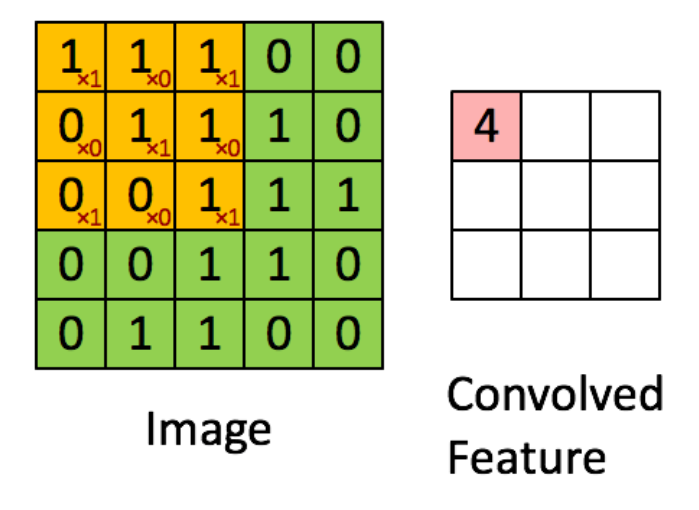
\includegraphics[scale=0.3]{../figs/convlayer5.png}
    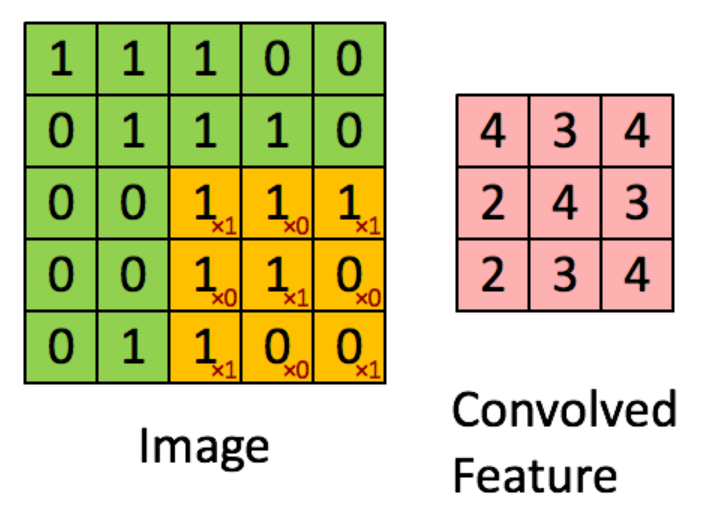
\includegraphics[scale=0.3]{../figs/convlayer4.png}
    \caption{Figure showing the application of a filter on an image comprised of binary values. Each value represents one pixel.}
    \label{fig:convlayer}
\end{figure}

To mitigate this, one can utilize something called \textbf{padding}. As the name implies, this simply means adding a border of $0$s around the input data, increasing the size of the image while not adding any disrupting features. This ensures that the output feature matrix does not shrink in size after one convolutional layer.

The process that actually decreases the size of the data set is called \textbf{pooling}, and is explained further in \cref{subsubsec:pooling}.

In short, a convolutional layer takes a multidimensional input and highlights different features in this input, yielding a matrix of similar or smaller size called an output feature matrix. This process can be done over several convolutional layers, resulting in more and more abstract output feature matrices as the network recognizes more and more complex patterns. These matrices are then pooled and can be processed by a DNN, as explained in \cref{subsubec:integration_dnn}.


\subsubsection{Pooling Layers}\label{subsubsec:pooling}
Pooling layers are somewhat similar to convolutional layers, but serve the simple purpose of reducing the size of the data into less granular information. A pooling layer passes over the data with a kernel and outputs some "pooled" version of it. This pooled version is often either the maximum value (called "max pooling") or the average value (called "average pooling") of the input data. The two concepts are outlined in \cref{fig:pooling}. The purpose of pooling layers are not to extract features, as convolutional layers do, but rather reduce the dimensionality of the data, in an effort to make it more manageable.

Pooling layers rely on the spatial correlation of the image. It assumes that the features of any particular pixel in the image is heavily correlated with the features of nearby pixels, and that they can together be approximated well when pooled together. Pooling layers also function as noise suppressor, as several pixels (or features) are gathered. Max pooling is often said to perform even better at suppressing noise, as it only extracts the highest value, possibly entirely removing potential noise, while average pooling will simply average over the noise.

\begin{figure}[H]
    \centering    
    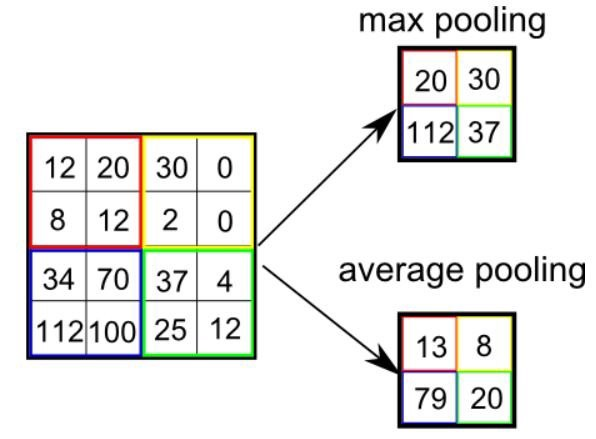
\includegraphics[scale=0.25]{../figs/pooling.png}
    \caption{Diagram illustrating max and average pooling, as employed in convolutional neural networks.}
    \label{fig:pooling}
\end{figure}

%-Max pooling take the max value in each equaly sliced piece of picture cake, reduces noise

%-Avg pooling averages the cake slice picture thing holy fuck i need to sleep now dont i

%-Takes big picture makes big picture small


\subsubsection{Dropout}
\label{sec:theory_dropout}
Dropout is a technique in neural network training, aimed at reducing the impact of overfitting on a network. During the training of the neural network, when performing the forward and backward propagation, a randomly selected fraction of nodes in each layer are "dropped" in each training batch. The dropped nodes are considered entirely absent from the network during that mini-batch, and the networks trains as if they didn't exist. For each mini-batch, a new set of nodes are selected. The dropout probability can different (or abscent) in any layer of the network. Figure \ref{fig:dropout} outlines the concept of dropout.

Dropout has been shown to reduce overfitting by forcing the network to distribute the learning more uniformly among the nodes, since no node can be guaranteed to be active during the any mini-batch. A more in-depth explanation and analysis of dropout can be found in \cite{dropout}.

\begin{figure}[H]
    \centering
    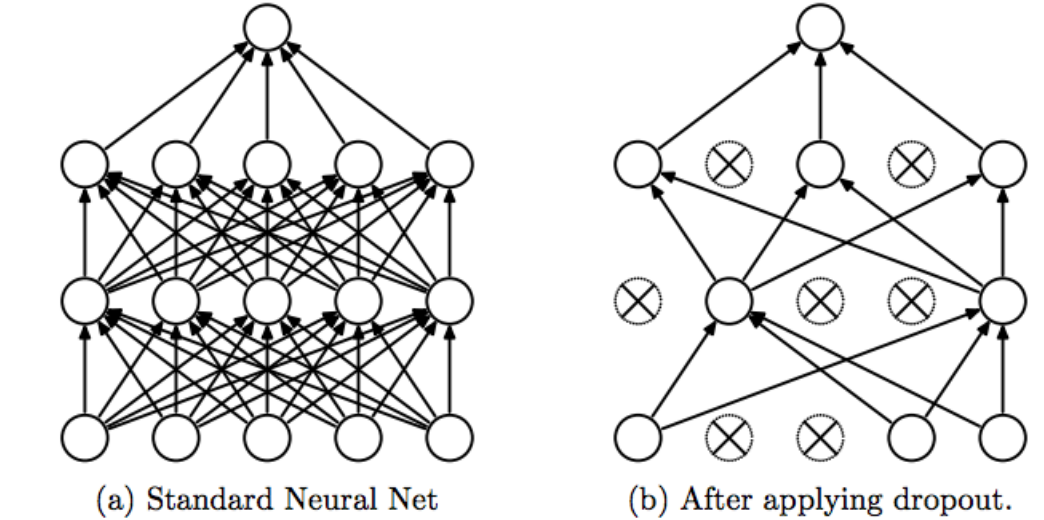
\includegraphics[scale=0.2]{../figs/dropout.png}
    \caption{Figure explaining the concept of dropout. A randomly selected fraction of nodes in each layer is neglected in each training batch. Figure found in \cite{dropout}.}
    \label{fig:dropout}
\end{figure}


\subsubsection{Integration with DNN}\label{subsubec:integration_dnn}
After several rounds of convolutional and pooling layers, the data in a convolutional neural network is flattened to 1D, and passed through a series of hidden dense layers, just like in an ordinary DNN. The data is at this point significantly reduced in size, and much more manageable for dense layers. Furthermore, the output from the last convolutional layers are often highly abstract features of the image. The dense layers can then perform the classification of the images on a highly abstracted feature set, instead of a very large set of pixels. This combination of layer types is very powerful. Figure \ref{fig:network} shows an example architecture of a full CNN, with convolutional layers, pooling, and fully connected layers toward the end.

\begin{figure}[H]
    \centering
    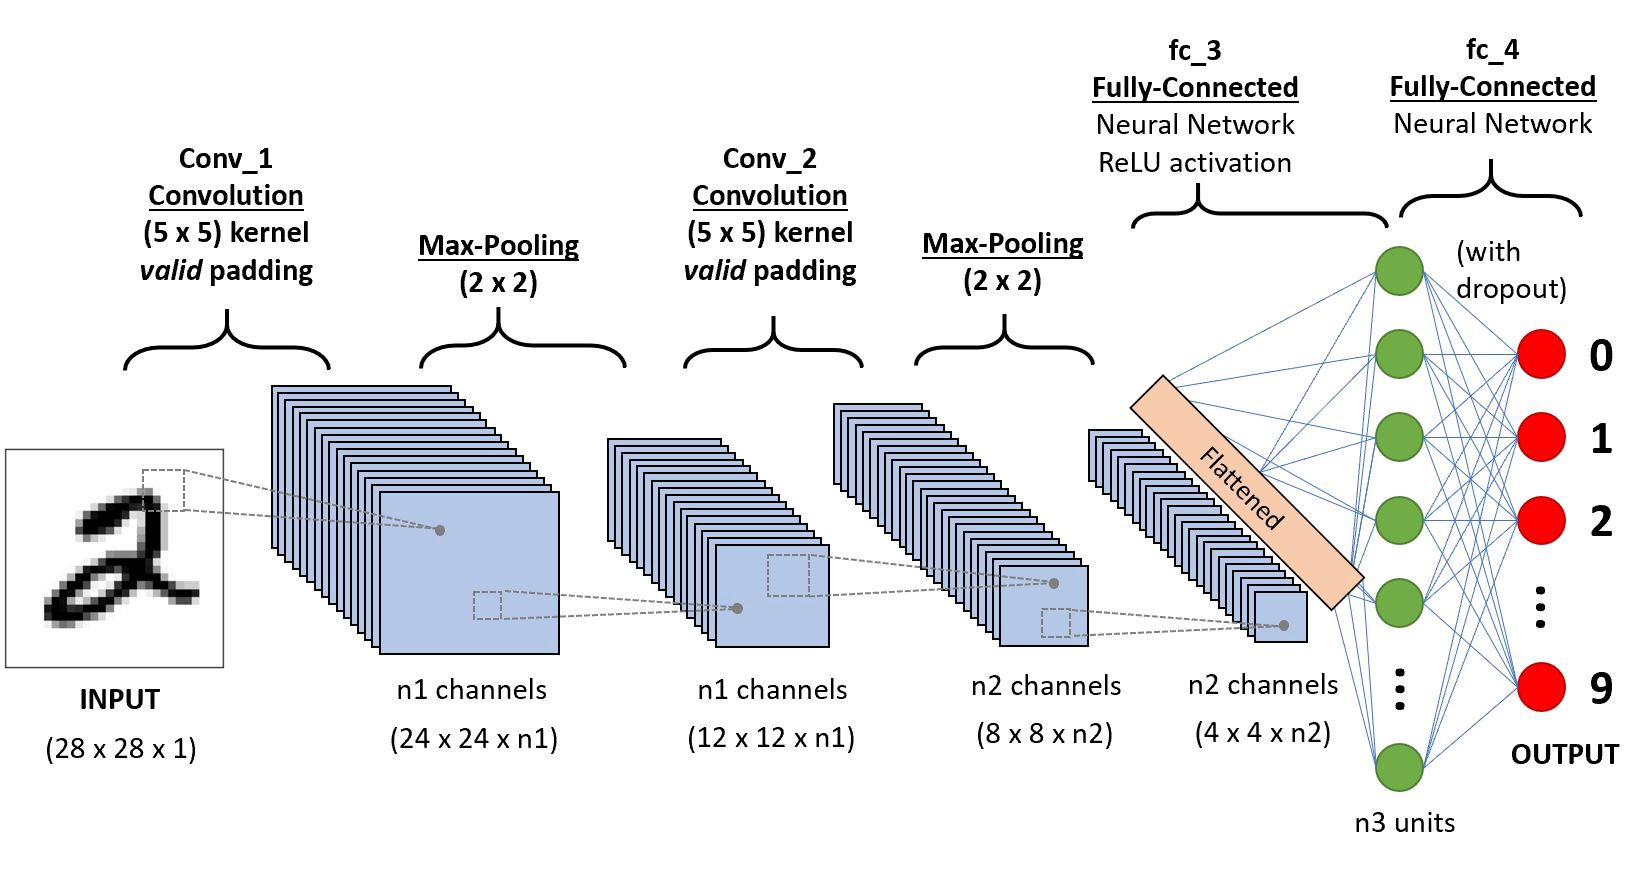
\includegraphics[scale=0.165]{../figs/network.jpeg}
    \caption{Diagram showing an example full network architecture for a CNN.}
    \label{fig:network}
\end{figure}

%-After all is said and pooled, the data is significantly decreased in size and much more managable for a DNN to deal with. So the CNN doesn't actually do the classification, right?? It just decomposes big images into smaller chunks of features, and then the DNN classifies those chunks of feateres as cats or dogs, instead of having to deal with the actual pictures..Right??

%-I hope this is correct because im really happy with the eyes+visual centre/neurons analogy and that all falls apart if this is not correct :(








% ███╗   ███╗███████╗████████╗██╗  ██╗ ██████╗ ██████╗ 
% ████╗ ████║██╔════╝╚══██╔══╝██║  ██║██╔═══██╗██╔══██╗
% ██╔████╔██║█████╗     ██║   ███████║██║   ██║██║  ██║
% ██║╚██╔╝██║██╔══╝     ██║   ██╔══██║██║   ██║██║  ██║
% ██║ ╚═╝ ██║███████╗   ██║   ██║  ██║╚██████╔╝██████╔╝
% ╚═╝     ╚═╝╚══════╝   ╚═╝   ╚═╝  ╚═╝ ╚═════╝ ╚═════╝
\section{Method}
\subsection{Data}
\label{subsubsec:Method/Data}
\begin{figure*}[ht]
    \centering
    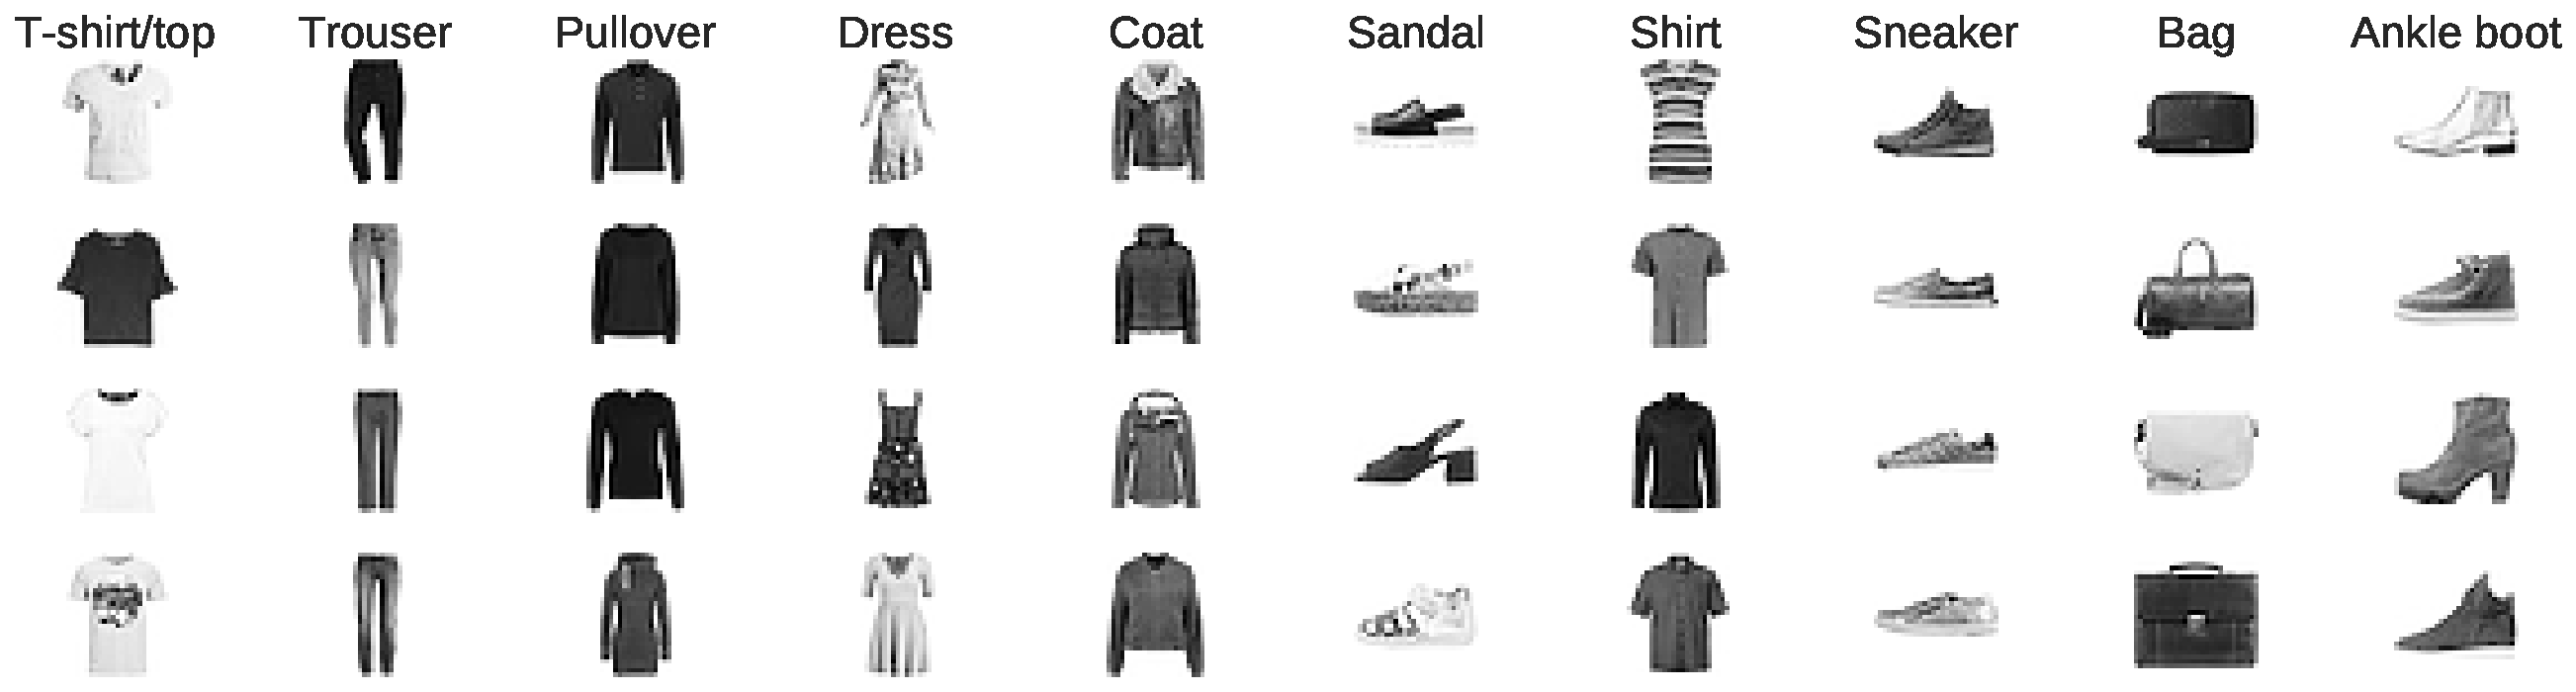
\includegraphics[scale=0.4]{../figs/fashion_examples.pdf}
    \caption{Figure showing 4 example images from each of the 10 categories in the fashion MNIST dataset. All images are 28x28 pixels of greyscale.}
    \label{fig:clothes}
\end{figure*}

We employed a dataset named "fashion MNIST", found on Kaggle (\url{https://www.kaggle.com/zalando-research/fashionmnist}). The dataset takes inspiration from the MNIST (Modified National Institute of Standards and Technology) database, which contains 70'000 images of handwritten digits, 0 through 9, in 28x28 pixel greyscale. MNIST is widely recognized  as the "Hello World" of deep learning. In the same spirit, our fashion MNIST dataset contains 70'000 28x28 greyscale images, classified into 10 categories. The images are gathered from the popular online clothing store Zalando, and is classified into 10 categories of clothing. Figure \ref{fig:clothes} show 4 randomly selected images from each category.

%The data required no further attention, in regards to cleaning, outlier removal, or otherwise. All the images was found to be centered, of good quality (their low resolution in consideration), and containing no other surprises.

In regards to cleaning the data, we initially found no distinct outliers or otherwise ill behaved images from our analysis. They were found to be centered, and of good quality (their low resolution in consideration), and so we continued using the full dataset.

\subsubsection{Choice of performance metric}
For all our models and analysis, we chose to go with the accuracy score as a performance metric. The accuracy score is simply defined as the fraction of predictions falling in the correct category, in other words
\begin{align}
    \text{Accuracy} = \dfrac{\text{Nr. of correct predictions}}{\text{Total nr. of predictions}}.
\end{align}
The accuracy score is often avoided because of its bias and poor performance when the data itself is biased. If a large portion of the data is contained in one category, any model guessing that every datapoint belongs to that category will perform rather well, using accuracy as a metric. Metrics like AUC ROC (Area Under the ROC Curve), are often used, faring better on biased data. However, our data is incredibly unbiased. Figure \ref{fig:label_dist} shows the distribution of categories among train, test, and validation data, revealing that all categories are extremely evenly represented in all datasets. For this reason, we saw no reason not to employ the accuracy score as our performance metric, as we saw no obvious disadvantages when the data is unbiased. The accuracy score also has the advantage of being very interpretable.


\begin{figure}[H]
    \centering
    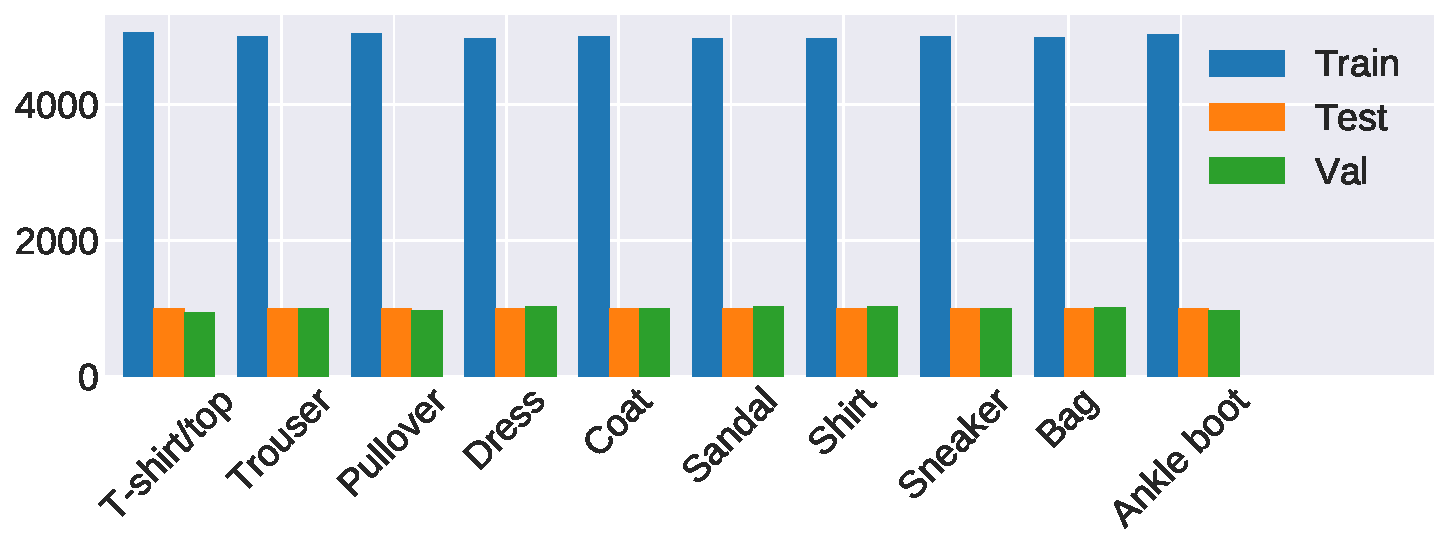
\includegraphics[scale=0.4]{../figs/label_distribution.pdf}
    \caption{Figure showing the number of label occurrences in both the training data of 50'000 images, and the test and validation datasets of 10'000 images each. The labels are observed to be extremely evenly distributed in all three datasets.}
    \label{fig:label_dist}
\end{figure}


\subsubsection{Train, test, and validation data}
Even when considerably downsized, images contain a lot of pixels, resulting in a large input layer. Image analysis is therefore extremely computationally demanding. In our case, the 28x28 grey-scale image left us with 784 nodes in the input layer. The size of the dataset, at 70'000 images, also posed a challenge. Limiting the computational requirements, where possible, was therefore a priority.

Ideally, we would like to have performed some sophisticated cross validation, like K-fold validation. We instead settled for splitting the data in a training set of 50'000 images, a testing set of 10'000 images, and a final validation set of 10'000 images. Every model was trained, tested, and validated, on the same set of images, increasing the comparability between models. The meaning of this is explained in the following section.


\subsubsection{Training, testing, and validation scheme}
\label{sec:method_train_test_val}
The purpose for including a validation set, in addition to a testing set, is for computational performance reasons. During the training of every model, the accuracy on the testing set was monitored. When the testing set reached its peak performance, the training of the model was stopped, and the networks was considered trained. Normally, this would be a big no-no, as the testing set is supposed to be off limits during training, and it should not directly impact the training. However, when evaluating the final performance of the models, we always use the accuracy score on the validation dataset, which is never touched during training. The main advantage of this approach is that the number of epochs to train the model is no longer a hyperparameter. Instead, the model trains until it is considered finished. Reducing the dimensionality of the hyperparameter space is vital for keeping computational costs low.



\subsection{Dense Neural Network}
As a reference to our convolutional neural network, we implemented an ordinary dense neural network. Dense networks don't usually perform particularly well on image classification, struggling from the fact that every node in every layer is interconnected, making it incapable of effectively exploiting the spatial information of the image. The network was implemented as a series of dense layers, each half the size of the previous one. By default, we implemented 5 dense layers, of [1024, 512, 256, 128, 64] neurons, in that order. Gradually decreasing the size of the layers throughout a dense neural network is common practice. The architecture of the network was, however, opened up to hyperparameter optimization.


\subsubsection{Implementation}
The network was built in Keras, a Python module, using Tensorflow as a backend. Keras offers extremely high levels of abstractions, allowing a network to be built and trained in a handful of lines. Using Keras, we built a general network building function, able of accepting hyperparameters, like network architecture, as input. The dense neural network implementation can be found in \texttt{Fashion\_DNN.ipynb}.

For all our networks, the widely recognized and well-performing Adam optimizer, introduced in \cite{adam}, was employed.



\subsubsection{Hyperparameter Optimization}
\label{sec:method_DNN_hp}
We decided on the learning rate, batch size, number of layers, and number of neurons per layer as hyperparameters to be optimized. The chosen hyperparameters can be found in \cref{tab:hp_table_DNN}. The number of neurons refer to the size of the first hidden layer. Subsequent hidden layers are always half the size of the previous layer.

Ideally, as it can be hard to predict how coupled the performance of certain parameters are, we would run every combination of hyperparameters. This would reveal any performance correlations. However, due to computational constrains, we limited ourselves to first running only every combination of the learning rates and batch sizes. This was done with 5 layers, with neuron size 1024, under the assumption that this represents a fairly average layer, and that the optimal learning rate/batch size combo of this network won't vastly differ from any of our other architectures.

With the results of the learning rates and batch sizes in mind, we ran every combination of number of layers and number of neurons with a batch size of 512, and a learning rate of $10^{-3}$. All runs were performed as described in \cref{sec:method_train_test_val}, using early stopping, and the accuracy score on validation data.

\begin{table}[H]
    \centering
    \begin{tabular}{l|l l l l l}
        Learning Rate & $10^{-2}$ & $10^{-3}$ & $10^{-4}$ & & \\
        \hline
        Batch Size & 8 & 64 & 512 & 4096 & \\
        \hline
        Nr. Layers & 1 & 2 & 4 & 6 & 10 \\
        \hline
        Nr. Neurons & 256 & 512 & 1024 & 2048 & 4096 \\
    \end{tabular}
    \caption{Table showing the listings of parameters used in hyperparameter optimization.}
    \label{tab:hp_table_DNN}
\end{table}



\subsection{Convolutional Neural Network}
As a more serious attempt at classifying the images, we implemented a convolutional neural network. Traditionally, they are known to far outperform dense neural networks on two dimensional data. CNNs have, to an even larger extent than dense networks, extremely much flexibility in model architecture. The convolutional layers themselves have both a filter size and a kernel size to consider, as outlined in \cref{sec:theory_conv_layers}. In addition, it is common to include techniques like regularization and dropout (outlined in \cref{sec:theory_dropout}). Dense layers are also often included towards the end of the network, further increasing the possible variations.

\subsubsection{Implementation}
Our convolutional networks were implemented in Keras, in similar fashion to the dense networks. Due to the enormous possible variety of network architectures, we decided upon a basic structure. The structure was inspired by the common convention of having several bulks of convolutional layers, each bulk with an increasing filter size, and a decreasing kernel size, with a pooling layer in between. A couple of dense layers follow.

Our networks can be divided into three bulks of layers, first, two bulks of  convolutional layers, and then two dense layers. The structure can be summarized as:

\begin{itemize}
    \item A first series of convolutional layers, with kernel size (5x5), some amount of dropout $d$, and $n$ filters. There is a number $m$ of these layers. They are followed by a max pooling layer, with (2x2) pooling.
    \item A second series of convolutional layers, with kernel size (3x3), some amount of dropout $d$, and $2n$ filters. There is also a number $m$ of these layers. They are followed by a (2x2) pooling, and a flattening.
    \item Two dense layers, with 256 nodes, and dropout rate $d$.
\end{itemize}

All layers was implemented with the ReLu activation function, and the Adam optimizer is used, just as in the dense network.

By default, we employed two of each convolutional layer ($m=2$), the first pair being of sizes 32, and the second pair of 64 ($n=32$), with a dropout of 20\% ($d=0.2$) on all layers. Deviations from this was explored in the hyperparameter optimization.

\subsubsection{Hyperparameter Optimization}
\label{sec:method_CNN_hp}
As with the dense network, hyperparameter optimization was performed on a selected set of parameters, shown in \cref{tab:hp_table_CNN}. The general outline of the network is outlined in the previous section. The number of layers refer to $m$, the number of convolutional layers in each of the bulks, and the number of neurons refer to $n$, the number of filters in the first bulk of convolutional layers, while the second bulk contains twice the number of filters, as outlined in the previous section. The strict setup is employed exactly to reduce the amount of hyperparameters, such that the optimization is actually feasible.

Just as in the dense network, the learning rates and batch sizes are ran independently, to preserve compute power, using the static $n=32$, $m=2$, and $d=0.2$. Then, all combinations of the number of layers, number of filters, and dropout, is run with a learning rate of $10^{-3}$ and a batch size of $1024$.

\begin{table}[H]
    \centering
    \begin{tabular}{l|l l l l}
        Learning Rate & $10^{-2}$ & $10^{-3}$ & $10^{-4}$ & \\
        \hline
        Batch Size & 8 & 64 & 512 & 4096 \\
        \hline
        Nr. Layers & 1 & 2 & 3 & \\
        \hline
        Nr. Filters & 16 & 32 & 64 & \\
        \hline 
        Dropout & 0 & 0.2 & & 
    \end{tabular}
    \caption{Table showing the listings of parameters used in hyperparameter optimization of the convolutional neural network.}
    \label{tab:hp_table_CNN}
\end{table}

\subsection{Human classification error}
Clothes are something familiar to all people. The ability to distinguish pants from coats and dresses from shirts is something most people learn at an early age. While looking through the data set and analyzing the results of our neural networks, a thought appeared: Could we outperform the networks accuracy score? If not, how does our performance compare to that of the neural network?

There are several factors at play here. The most obvious is that, while human brains have several years of training in classifying items of clothing, this classification is usually not done on downsized grayscale images. The neural networks are however trained on exactly this type of data, and might be able to see patterns we are too biased to see. 

Which is an important second point: bias. The data set we're working with has initially been classified by a person, and people have biases and preconceived notions of what fits in which category. One might not agree on the differences between tops, shirts and pullovers, for example, especially when only presented with a low resolution greyscale image.

Lastly, people get bored and distracted. Tell a computer to classify thousands of items, and it will duly do so. Tell a person to do the same, and they might have some objections. Zoning out, becoming impatient and accidentally misslabeling items are sources of human error one will not find in an artificial neural network.

To make the classification process as enjoyable as possible for us, which should mitigate some of the aforementioned errors due to boredom and distraction, we tried to implement a touch of gamification. We wrote a small script that picked a random picture from the pool of images, where we then had to choose what we thought was the proper category form a list of all the possible categories. If we chose right, we got a nice green "Hooray!" message, and if we chose wrong we got a red "Booh!" message telling us what the proper category was. This way it was possible to immediately learn form our mistakes and learn what defined each category. We also continuously kept track of both the cumulative accuracy, giving us direct feedback at all times over how well we we're doing. We ended up categorizing 1000 images each. Both the cumulative and running accuracy was recorded, for later analysis.



% ██████╗ ███████╗███████╗██╗   ██╗██╗  ████████╗███████╗
% ██╔══██╗██╔════╝██╔════╝██║   ██║██║  ╚══██╔══╝██╔════╝
% ██████╔╝█████╗  ███████╗██║   ██║██║     ██║   ███████╗
% ██╔══██╗██╔══╝  ╚════██║██║   ██║██║     ██║   ╚════██║
% ██║  ██║███████╗███████║╚██████╔╝███████╗██║   ███████║
% ╚═╝  ╚═╝╚══════╝╚══════╝ ╚═════╝ ╚══════╝╚═╝   ╚══════╝

\section{Results}
\subsection{Dense Neural Network}
Our initial qualified guess at a dense neural network architecture gave a validation accuracy score of 0.899. The train and test accuracies over epochs is plotted in \cref{fig:DNN_epochs}. As we can see, very few epochs was needed to achieve good accuracies of around 90\% for the testing set. The training set, however, keeps increasing, reaching virtually 100\%. This does interestingly enough not negatively impact the testing set, which remains at virtually constant accuracy even as the network heavily overfits on the training data.


\subsubsection{Hyperparameter Optimization}
Running the network with the hyperparameters described in \cref{sec:method_DNN_hp}, the results are seen in \cref{fig:DNN_hp1} and \cref{fig:DNN_hp2}. In \cref{fig:DNN_hp1} we see the accuracy scores on validation data as a function of learning rate and batch size. It's evident that the network performs best with a relatively low learning rate, combined with a small batch size. All networks with learning rates smaller or equal to $10^{-3}$, combined with batch sizes smaller or equal to $512$, performed acceptably well. The absolutely worst results arrive with the lowest batch size, combined with the highest learning rate. This is especially interesting considering that the best results were also achieved with the same batch size. This is, however, not entirely surprising. A small batch size means that individual images get much more attention when calculating the gradient. Combined with a high learning rate, niche features in individual images might be overlearned, at the expense of the networks general performance. This effect can be overcome either by increasing the batch size, or decreasing the learning rate, exactly as we observe in \cref{fig:DNN_hp1}.

Figure \cref{fig:DNN_hp2} shows the networks performance as a function of number of layers and number of neurons per layer. The performance difference between the networks is small, but some of the best results are seen by the wide one-layer networks, of size 1024, 2048, and 4096. The trend is, however, very weak, and one could also conclude that most networks fall within the margin of error. Either way, the best network comes out at an accuracy of $90.9\%$.

\begin{figure}[H]
    \centering
    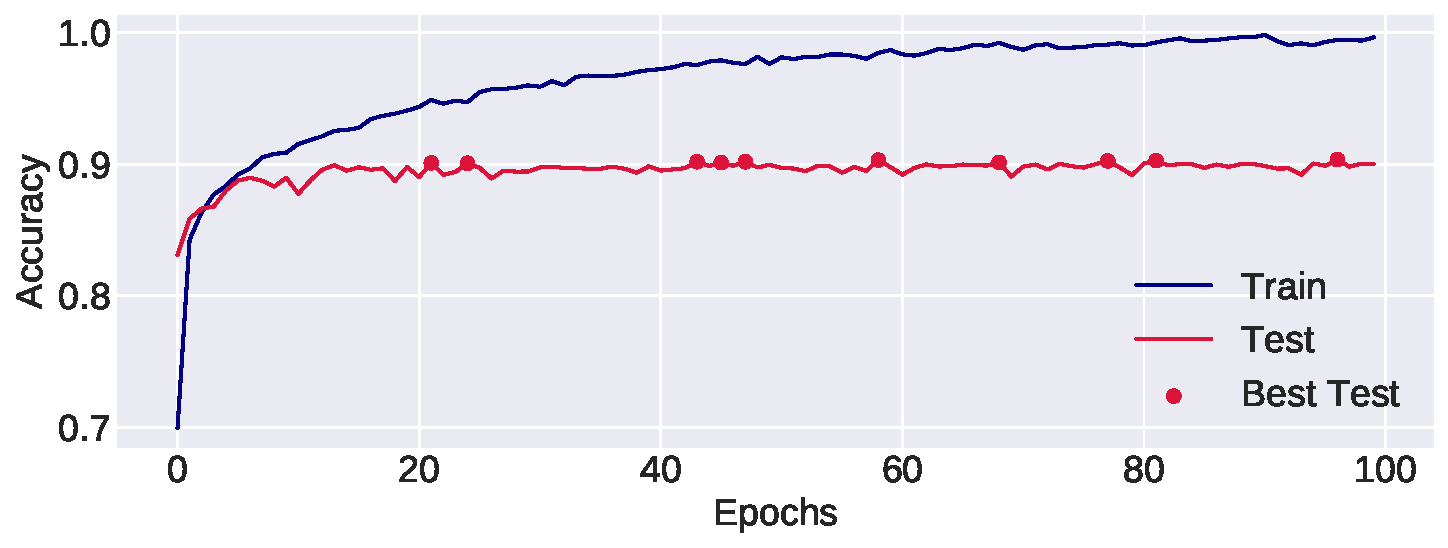
\includegraphics[scale=0.4]{../figs/DNN_epochs.pdf}
    \caption{Plots showing the training and testing accuracy of a dense neural network on the fashion data. The 10 best test accuracies are marked as points. While the training accuracy increases constantly, reaching virtually 100\% after ~90 epochs, the testing accuracy levels out at around 90\% after ~20 epochs. The network has 5 layers of sizes [1024, 512, 256, 128, 64], in that order, with learning rate $10^{-3}$ and batch size 1024.}
    \label{fig:DNN_epochs}
\end{figure}

\begin{figure}[H]
    \centering
    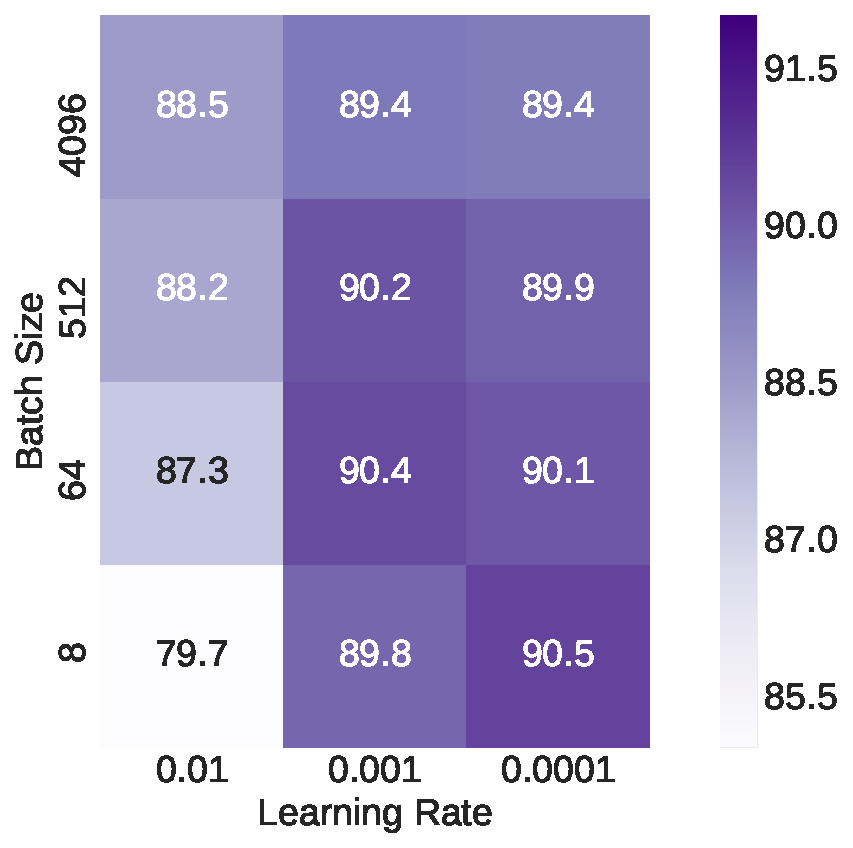
\includegraphics[scale=0.4]{../figs/DNN_lr_batchsize_heatmap.pdf}
    \caption{Heatmap showing the accuracies of the dense neural network with varying learning rate and batch size. The best network has a learning rate of $10^{-3}$, and a batch size of 8, performing an accuracy of 90.54\%. All networks have 5 layers, with [1024, 512, 256, 128, 64] neurons, respectively.}
    \label{fig:DNN_hp1}
\end{figure}

\begin{figure}[H]
    \centering
    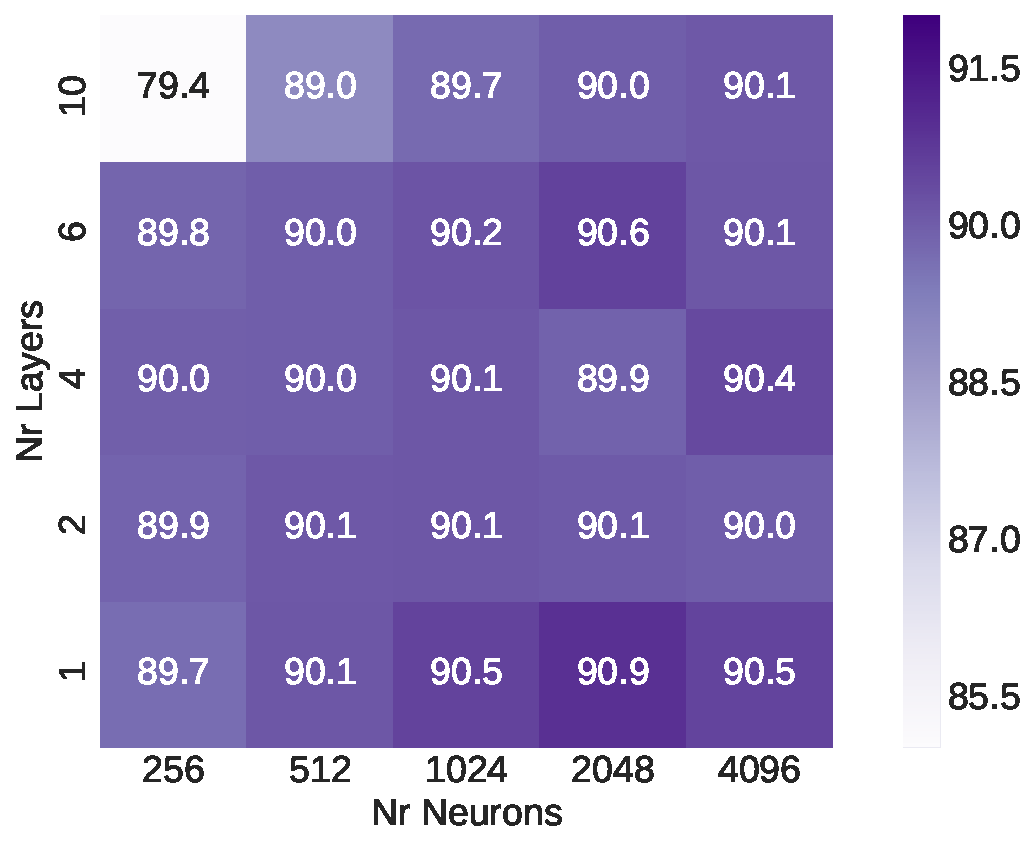
\includegraphics[scale=0.4]{../figs/DNN_layers_neurons_heatmap.pdf}
    \caption{Heatmap showing the accuracies of the dense neural network with varying number of layers, and neurons per layer. The best network has 1 layer, with 2048 neurons, performing an accuracy of 90.91\%. All networks have a learning rate of $10^{-3}$, and 512 in batch size. The number of neurons indicate the first and biggest layer, with successive layers each having half the number of the previous.}
    \label{fig:DNN_hp2}
\end{figure}


\subsection{Convolutional Neural Network}
\subsubsection{Hyperparameter Optimization}
The hyperparameter optimization of learning rate and batch sizes show much of the same trends as they did for the dense network, as seen in \cref{fig:CNN_lr_batch_heatmap}. High learning rate with low batch sizes are a bad combination, while the best combination lies as a learning rate of $10^{-3}$ with a batch size of 256. This performed an accuracy of 93.50\%.

The performance of different network architectures, with and without dropout, is shown in \cref{fig:CNN_network_size_heatmap}. We see that, for each dropout scenario, all networks fall within a margin of 1\% of each other. This makes it challenging to draw conclusions with strong statistical significance about the network arcitechture. It does seem like bigger filter sizes perform somewhat stronger, and the best network clocked in at 93.47\%, with filter size 64, 2 layers per bulk, and dropout of 20\%. It's also worth noting that this is actually lower than the best network we got in the learning rate / batch size optimization, of 93.50\%. The exact same network performed an accuracy of 92.3\% during this run. Even though we are training, testing and validating on the same datasets twice, it is obvious that the networks performance has a slight variance, in this specific case of 0.2\%. Individual results with differences below something like 0.5\% should probably be taken with a grain of salt.

Even though the network architecture didn't seem majorly impactful, the dropout seems to systematically improve the performance. Comparing the two heatplots in \cref{fig:CNN_network_size_heatmap}, the networks with 20\% dropout scores ~0.5-1\% higher on every single network, without exception. This difference is further illustrated in \cref{fig:CNN_dropout_boxplot}, showing a boxplot of the performance with and without dropout. 

\begin{figure}
    \centering
    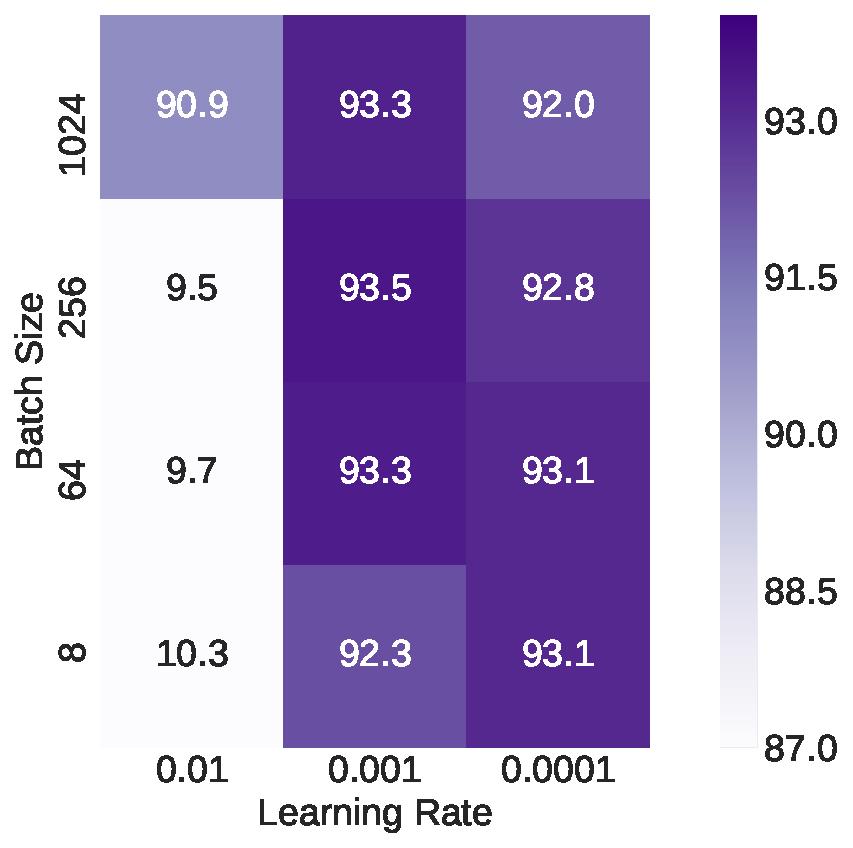
\includegraphics[scale=0.4]{../figs/CNN_lr_batchsize_heatmap.pdf}
    \caption{Heatmap showing the accuracy scores on validation data of CNN models with different batch sizes and learning rates. All models use models with filter size 32 and 2 layers per bulk, as described in \cref{sec:method_CNN_hp}.}
    \label{fig:CNN_lr_batch_heatmap}
\end{figure}

\begin{figure}[H]
    \centering
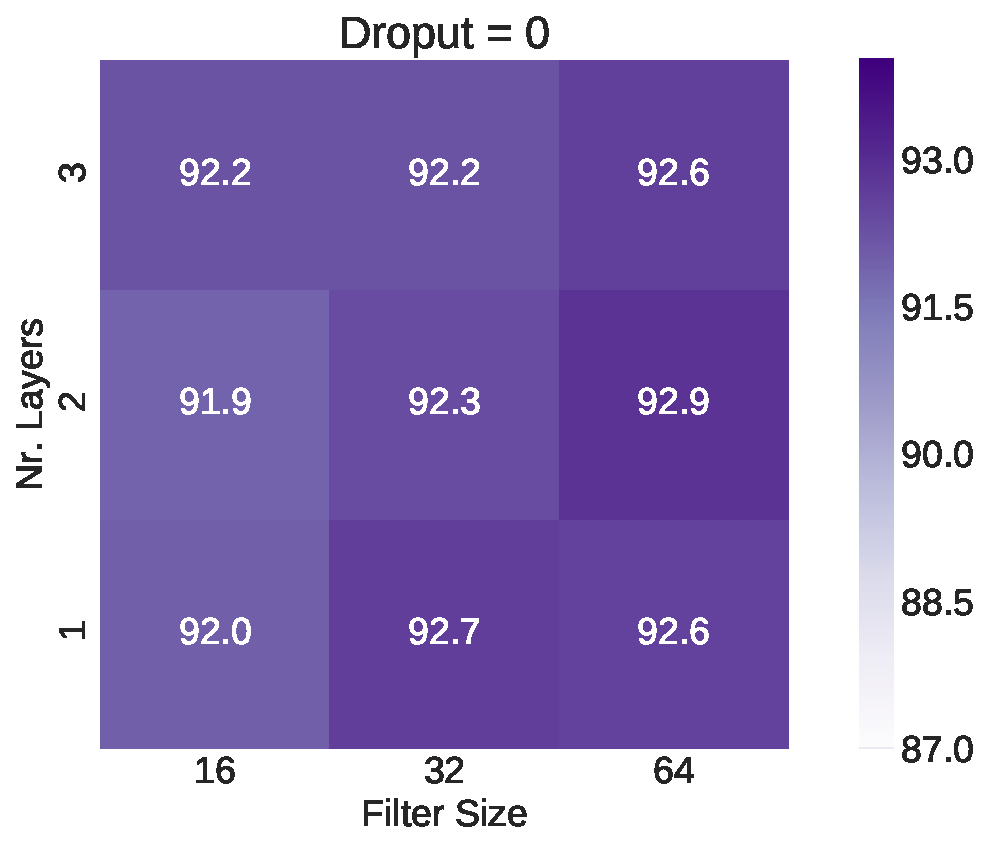
\includegraphics[scale=0.4]{../figs/CNN_network_size_0d.pdf}
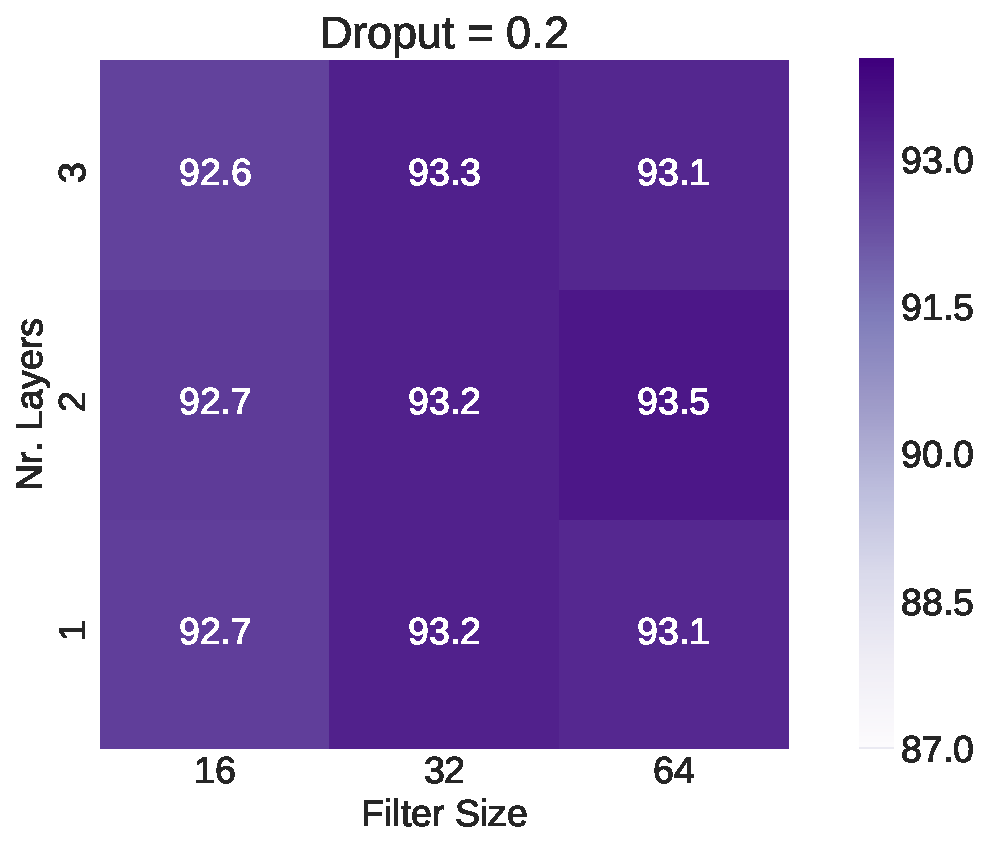
\includegraphics[scale=0.4]{../figs/CNN_network_size_20d.pdf}
    \caption{Heatmaps showing the accuracy scores on validation data of CNN models with no dropout (top) and 20\% dropout (bottom) over different number of layers and filters. All models use a learning rate of $10^{-3}$, and a batch size of 256.}
    \label{fig:CNN_network_size_heatmap}
\end{figure}

\begin{figure}[H]
    \centering
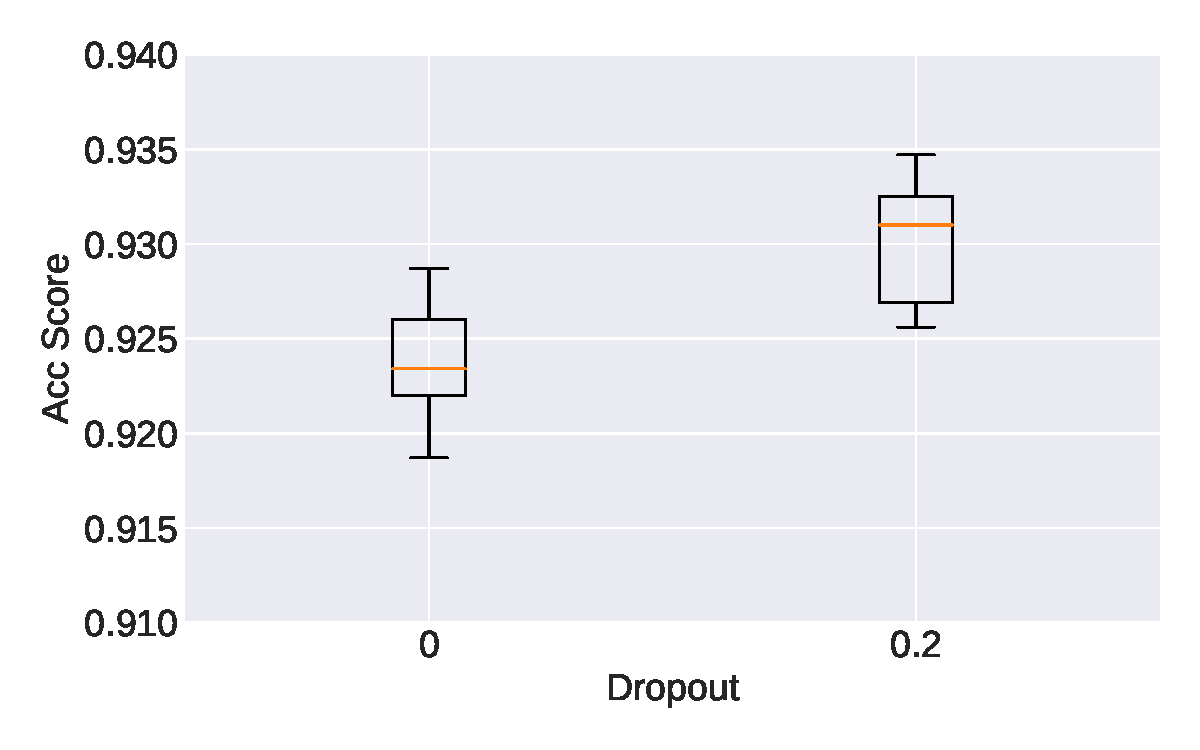
\includegraphics[scale=0.4]{figs/CNN_dropout_boxplot.pdf}
    \caption{Boxplot showing the distribution of accuracy scores on validation data for all the CNNs in \cref{fig:CNN_network_size_heatmap}, for dropout 0\% and 20\%.}
    \label{fig:CNN_dropout_boxplot}
\end{figure}



\subsection{Final performance analysis}
The best performing CNN model from our hyperparameter analysis had a batch size of 256, a learning rate of $10^{-3}$, 2 convolutional layers per batch, and a filter size of 32. Table \ref{tab:performance_table} shows the accuracy of this CNN across all categories. This reveals a lot about what the network is struggling with. A handful of the categories have almost perfect scores, trailing 100\% by only a few percentage points. However, T-shirt/top, pullover, dress, coat, and shirt all fall near or below 90\%. Figure \ref{fig:wrong_iamges} gives a pretty clear understanding of why this is. The aforementioned categories look a lot alike, and many of these images might even be wrongly categorized by a human. There are also signs of images that doesn't follow the convention of the others. We observe one of the images containing a model wearing a coat. It was, to our great amusement, categorized as a bag. The dataset might contain more such outliers which we didn't catch in our initial data analysis discussed in \cref{subsubsec:Method/Data}, which will understandably confuse our network. Some other examples of such outliers are uneven reflections and rotated cloths.


\begin{table}[H]
    \centering
    \begin{tabular}{l r}
        \textbf{Category} &  \textbf{Accuracy} \\
        \hline
     T-shirt/top &      \color{red} 0.86 \\
        \hline
         Trouser &      1.00 \\
        \hline
        Pullover &      \color{red} 0.89 \\
        \hline
           Dress &      \color{red} 0.91 \\
        \hline
            Coat &      \color{red} 0.88 \\
        \hline
          Sandal &      0.99 \\
        \hline
           Shirt &      \color{red} 0.84 \\
        \hline
         Sneaker &      0.96 \\
        \hline
             Bag &      0.99 \\
        \hline
      Ankle boot &      0.98 \\
      \hline
    \end{tabular}
    \caption{Table showing accuracies across categories of the best-performing CNN model. Sub-95\% performance categories are marked in red.}
    \label{tab:performance_table}
\end{table}


\begin{figure*}[ht!]
    \centering
    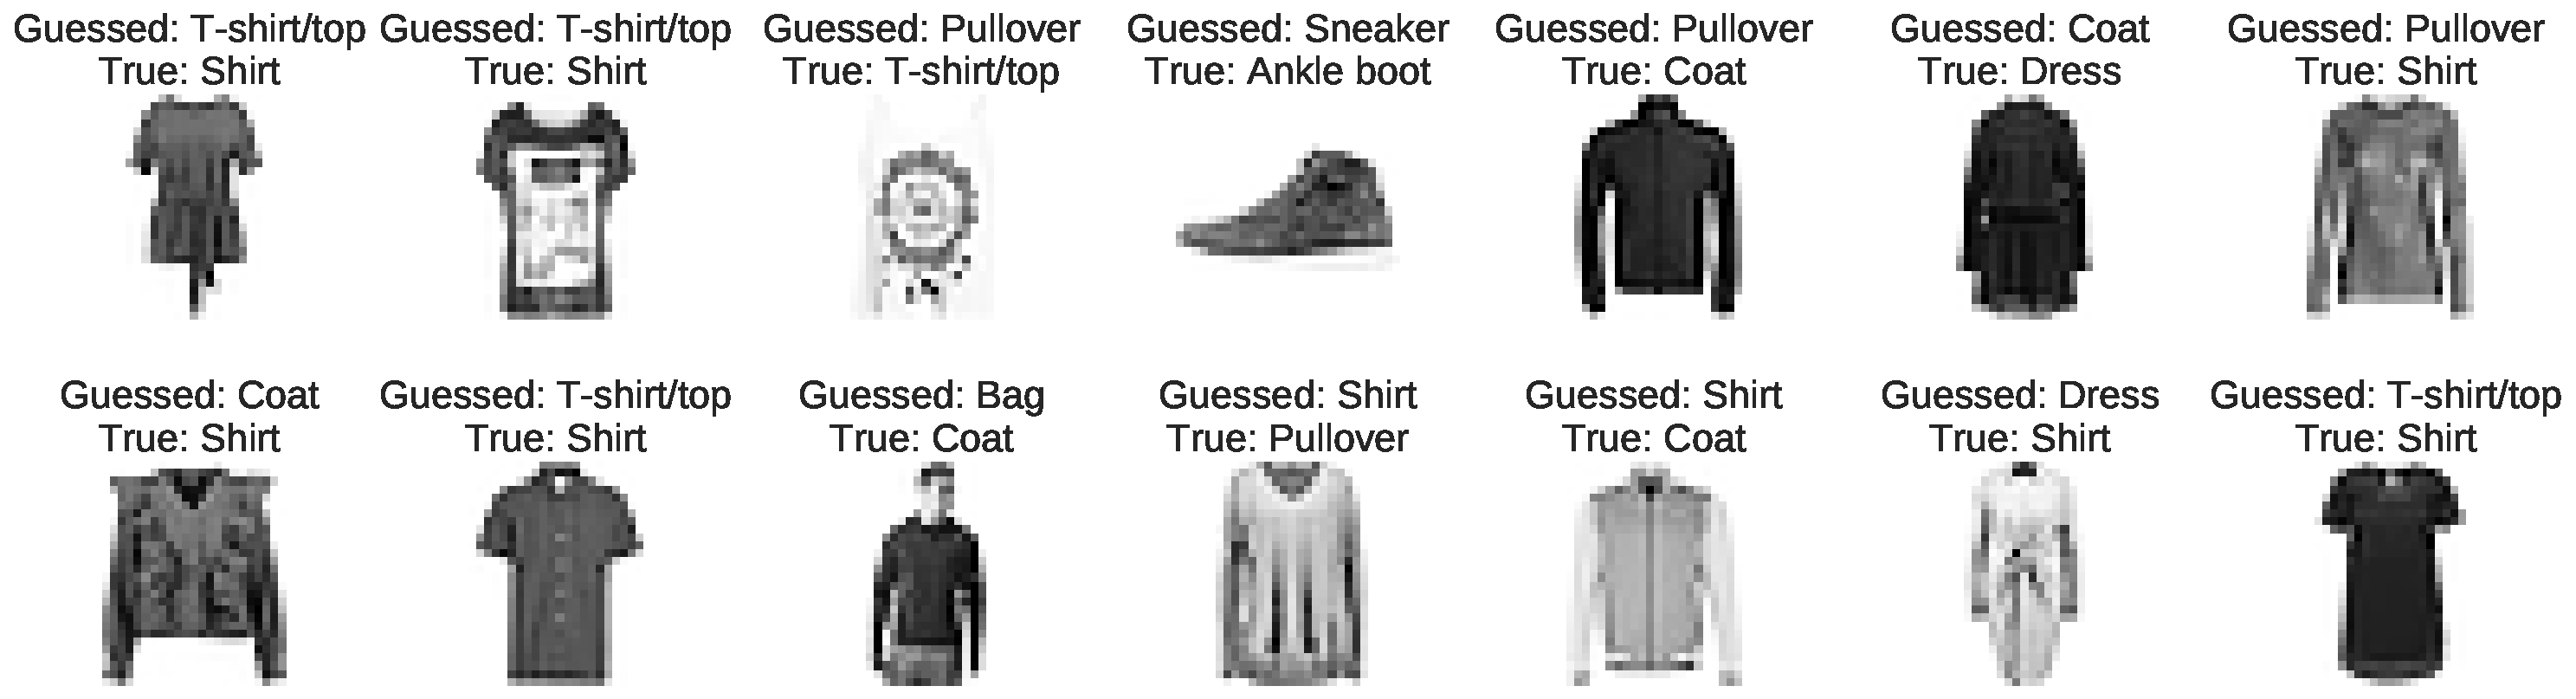
\includegraphics[scale=0.4]{figs/wrong_images.pdf}
    \caption{A random selection of the wrongly categorized images. Both the true labeled category and the predicted category are shown.}
    \label{fig:wrong_iamges}
\end{figure*}



\subsection{Human Performance}
In \cref{fig:human_cumulative} we see the cumulative average accuracy for the three human classification runs, with each of the three authors. There are several interesting things happening here. First and foremost, this clearly shows that both the DNN and CNN outperform human classification significantly. While both networks with optimal hyper parameters yield accuracy scores over 90\%, all three authors performances converges to $84.5(\pm 0.5)\%$. While a sample set of three people isn't really enough to say anything definite, it is really interesting that all authors converge towards the same accuracy score, especially considering how different each perform in the beginning.

The differences at the beginning of the classification process is interesting in itself, and it illustrates how a person might be better than an ANN in the beginning due to already being able to differentiate shoes from trousers and bags from sweaters. But as mentioned, this initial advantage does not beat the ANNs later on. Figure \cref{abend:human_error} in \label{abend:human_error} shows the running average accuracy, which indicates all three participants oscillating around the same accuracy score, at least after an initial couple of hundred images.

\begin{figure}[H]
    \centering
    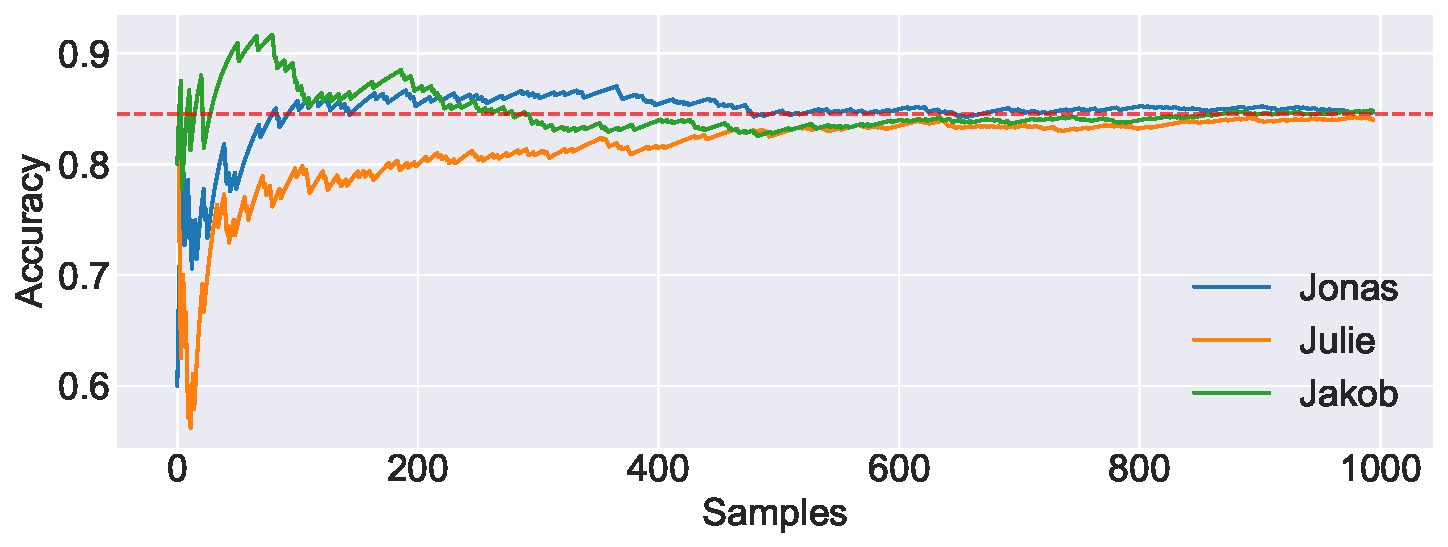
\includegraphics[scale=0.4]{figs/human_cumulative.pdf}
    \caption{Plot showing the cumulative average accuracy of the three authors categorization runs of 1000 samples from the validation set. While the initial "learning" rate for each of the authors are quite different, the general trend towards the end of the 1000 samples is clear, averaging out at $84.5\%$ as indicated by the red dashed line.}
    \label{fig:human_cumulative}
\end{figure}

A table over the average accuracy in each category can be seen in \cref{tab:human_performance_table}. The table also contains the CNN accuracies from \cref{tab:performance_table}, for comparison. The neural network and the humans appear to struggle with the same categories, which seems natural. The network also notably outperforms the humans in every single category. We also see that both the authors and the neural network struggle with clothes for the upper body. Interestingly, the CNN performed very well on sneakers and ankle boots, whereas the authors struggled with these categories as well. Whether or not this is a result of the CNN seeing patterns we aren't seeing, or the three of us being abnormally bad at distinguishing footwear is hard to answer. It would have been interesting to have more people doing the classification to see if this is just a weird quirk or an actual trend in human classification of this particular data set.

\begin{table}[H]
    \centering
    \begin{tabular}{l r r}
        \textbf{Category} &  \textbf{Human Acc.} & \textbf{CNN Acc.}  \\
        \hline
     T-shirt/top &      \color{red} 0.81 & \color{red} 0.86 \\
        \hline
         Trouser &      0.99 & 1.00 \\
        \hline
        Pullover &      \color{red} 0.73 & \color{red} 0.89 \\
        \hline
           Dress &      \color{red} 0.82 & \color{red} 0.91 \\
        \hline
            Coat &      \color{red} 0.73 & \color{red} 0.88 \\
        \hline
          Sandal &       0.96 & 0.99 \\
        \hline
           Shirt &      \color{red} 0.68 & \color{red} 0.84 \\
        \hline
         Sneaker &      \color{red}0.83 & 0.96 \\
        \hline
             Bag &      0.98 & 0.99 \\
        \hline
      Ankle boot &      \color{red} 0.92 & 0.98 \\
      \hline
    \end{tabular}
    \caption{Table showing the average accuracies across each category of the three authors categorization runs of 1000 samples from the validation set each, as well as the accuracy scores of the best-performing CNN. Sub-95\% performance categories are marked in red. The CNN performs better in all the categories.}
    \label{tab:human_performance_table}
\end{table}



%  ██████╗ ██████╗ ███╗   ██╗ ██████╗██╗     ██╗   ██╗███████╗██╗ ██████╗ ███╗   ██╗
% ██╔════╝██╔═══██╗████╗  ██║██╔════╝██║     ██║   ██║██╔════╝██║██╔═══██╗████╗  ██║
% ██║     ██║   ██║██╔██╗ ██║██║     ██║     ██║   ██║███████╗██║██║   ██║██╔██╗ ██║
% ██║     ██║   ██║██║╚██╗██║██║     ██║     ██║   ██║╚════██║██║██║   ██║██║╚██╗██║
% ╚██████╗╚██████╔╝██║ ╚████║╚██████╗███████╗╚██████╔╝███████║██║╚██████╔╝██║ ╚████║
%  ╚═════╝ ╚═════╝ ╚═╝  ╚═══╝ ╚═════╝╚══════╝ ╚═════╝ ╚══════╝╚═╝ ╚═════╝ ╚═╝  ╚═══╝
\section{Conclusion}
In this project we have explored one of the most promising areas of machine learning, namely image classification problems using neural networks. We have compared the more traditional dense neural network model to convolutional neural networks, renown for its great performance on two-dimensional data. The networks were tested on a 10 category set of 60'000 28x28 grayscale images, called Fashion-MNIST. Some hyperparameter optimization was performed for both network types, but computational requirements due to data size and network architecture restricted the number of parameters. The networks were also compared to the classification performance of the authors themselves.

% In the past the traditional multilayer perceptron (MLP), or dense neural networks, were used for image recognition. These methods suffer from the curse of dimensionality, where the number of parameters and weights quickly skyrocket already for small to medium images because of the full connectivity between each layer. This imposes a large requirement for computational power, as we have faced in this project even with small greyscale images. The introduction of convolutional neural networks revolutionized the image classification field, being able to utilize the spatial correlation in a two dimensional image instead of correlating each pixel to every other pixel. While still requiring high computational power, by the designers choice of filters with shared weights, pooling and dropout layers together with the rise of computational power the last decades we are able to handle problems which before were not possible.

% Here we have delved into one of the most popular datasets used for benchmarking neural network algorithms, the Fashion-MNIST set which serves as a replacement or supplement to the widely used original MNIST digits data. Before comparing the two networks we have to mention the problem of complexity and run time. This was problematic, as the sheer complexity of the CNN makes it hard to correlate to the training time of the more straight forward DNN. In order to make a fair comparison we aimed to have the run time of the two networks approximately on the same scale. 

Our initial dense neural network setup, using 5 layers of sizes 1024 decaying to 64, with a learning rate of $10^{-3}$ and a batch size of 1024, gave the quite decent accuracy score of $0.899$ on the validation data. Hyperparameter optimization on the DNN gave a best accuracy score of $0.909$, gained with 1 layer of 2048 neurons, with a learning rate of $10^{-3}$ and a batch size of 512. Most of the dense networks performed more or less the same, within margin of error, but seemed to somewhat favor shallow and wide networks. There was also a preference for lower learning rates and batch sizes.

The best-performing convolutional neural network clocked in at an accuracy of $93.50\%$, which corresponds to around a $30\%$ lower error rate than the best-performing DNN. This score is in line with some of the top voted kernels on Kaggle, \cite{Kaggle_kernel} as a good example, also for further reading. The networks with larger convolutional filter sizes generally performed better, while the number of convolutional hidden layers were less relevant. We also found that including a $20\%$ dropout on all layers improved the accuracy on all networks by around $1\%$.

Although a $30\%$ reduction in error rate is respectable, it was perhaps less that expected, and the difference between the convolutional and dense network architectures were smaller than expected. Some of the reason for this is undoubtedly the small dimensionality of the input images. The larger and more complex the images are, the more a dense network will struggle to classify them. Our images were of very low resolution, and in grayscale, both probably contributing to the small difference between the networks.

Finally, we saw that the human accuracy (as performed by the authors) on the dataset was lower than that of both the networks, at an average of $84.5\%$. The accuracy scores of all three participants were also very similar, agreeing to within a percentage point, pointing towards a surprisingly constant human error rate on the dataset. The network was also found to outperform the human participants in every single category. It is not particularly common to see neural networks outperform humans at image classification, making this a very interesting observation. It can probably be attributed to the low resolution of the images, which we, as humans, are not used to, while the network seems quite content with it. A lot of the categories were also somewhat vague, and humans carry a bias in what we imagine these categories to mean, while the network trains itself from a completely unbiased standpoint.

% Finally we would like to comment on the possibility of approaching an accuracy of one, not missclassifying any of the images. From our final analysis we see that our model actually is approaching this ideal for some of the categories, while the five similar categories for torso clothing is weighing down the mean score. Inspecting \cref{fig:wrong_iamges} we concluded that some of these categories would be hard to distinguish even for a human, and so we also compared our network to the authors classification errors of 1000 sample images. While the amusing errors like a coat being categorised as a bag is unlikely by human inspection, determining if some of these down scaled pictures are supposed to represent a T-shirt/top or just a shirt is no easy task. Interestingly we saw that the network was superior to our own classification in every single category, especially the aforementioned problematic categories, with our combined average error rate of $84.5\%$ across all categories. While this in theory does not rule out the possibility of a network performing at $100\%$ accuracy, it is unreasonable to expect the supervised artificial neural network algorithms to perform much better than the ones we have presented here with our limited computational power.

\subsection{Future Prospects}
In this project our biggest challenge was facing the limiting computational power available. This limited the types of images we were able to categorize, as well as the training time and the time spent on hyperparameter optimization. As we have seen our networks performing quite well, actually outperforming humans, it would be really interesting to unleash them on more interesting datasets, as well as spending even more time on the optimization to stretch the performance to the highest limits. While the dominance of convolutional neural networks in image recognition is evident, they also require huge amounts of computational power.




%  █████╗ ██████╗ ██████╗ ███████╗███╗   ██╗██████╗ ██╗██╗  ██╗
% ██╔══██╗██╔══██╗██╔══██╗██╔════╝████╗  ██║██╔══██╗██║╚██╗██╔╝
% ███████║██████╔╝██████╔╝█████╗  ██╔██╗ ██║██║  ██║██║ ╚███╔╝ 
% ██╔══██║██╔═══╝ ██╔═══╝ ██╔══╝  ██║╚██╗██║██║  ██║██║ ██╔██╗ 
% ██║  ██║██║     ██║     ███████╗██║ ╚████║██████╔╝██║██╔╝ ██╗
% ╚═╝  ╚═╝╚═╝     ╚═╝     ╚══════╝╚═╝  ╚═══╝╚═════╝ ╚═╝╚═╝  ╚═╝
\onecolumn
\bibliography{ref}
\newpage
\begin{appendices}
\section{Hot dog, not hot dog}
For further clarification, see \url{https://www.youtube.com/watch?v=pqTntG1RXSY}
\begin{figure}[H]
    \centering
    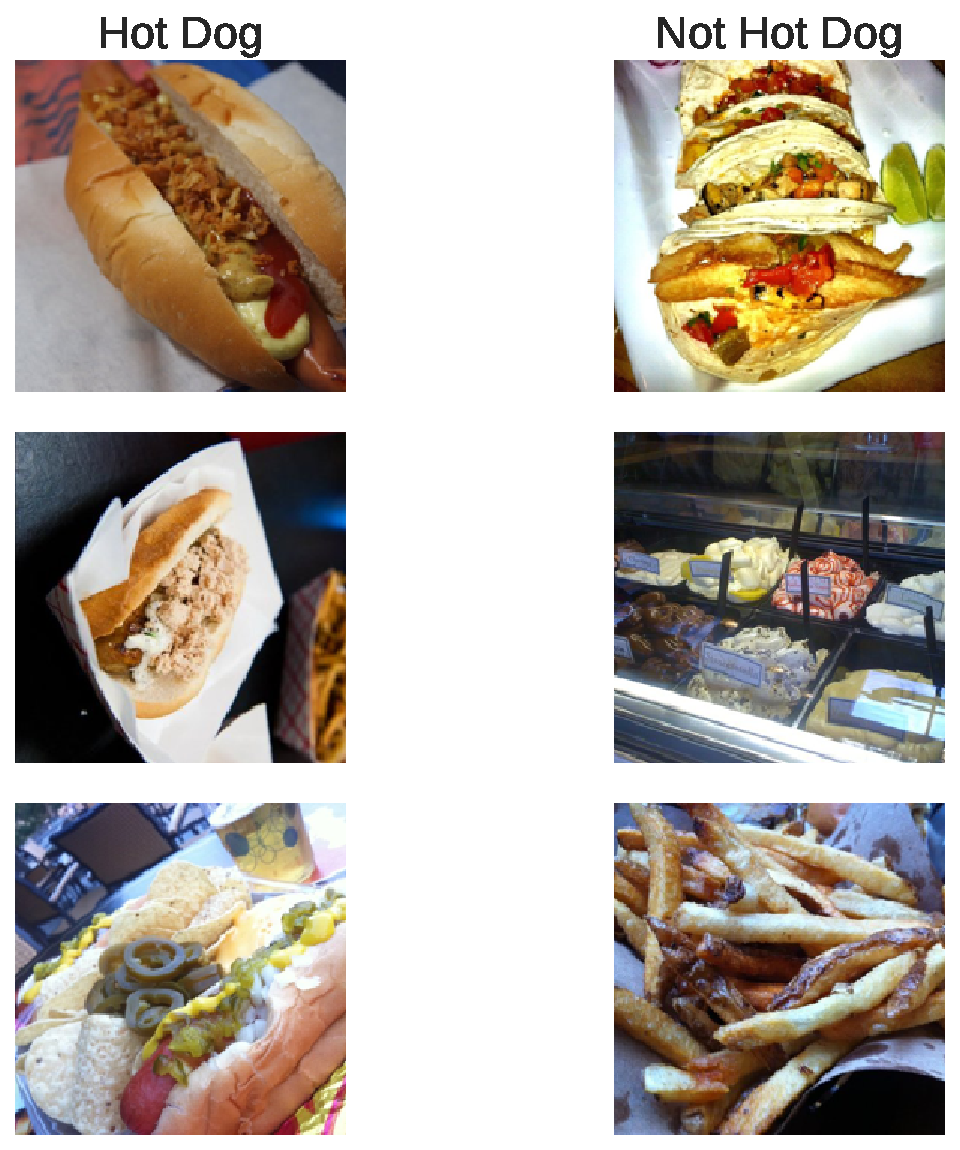
\includegraphics[scale=0.4]{figs/hotdog_examples.pdf}
    \caption{Images showing randomly selected hot dog and not hot dog images.}
    \label{fig:hotdog_examples}
\end{figure}

\begin{figure}[H]
    \centering
    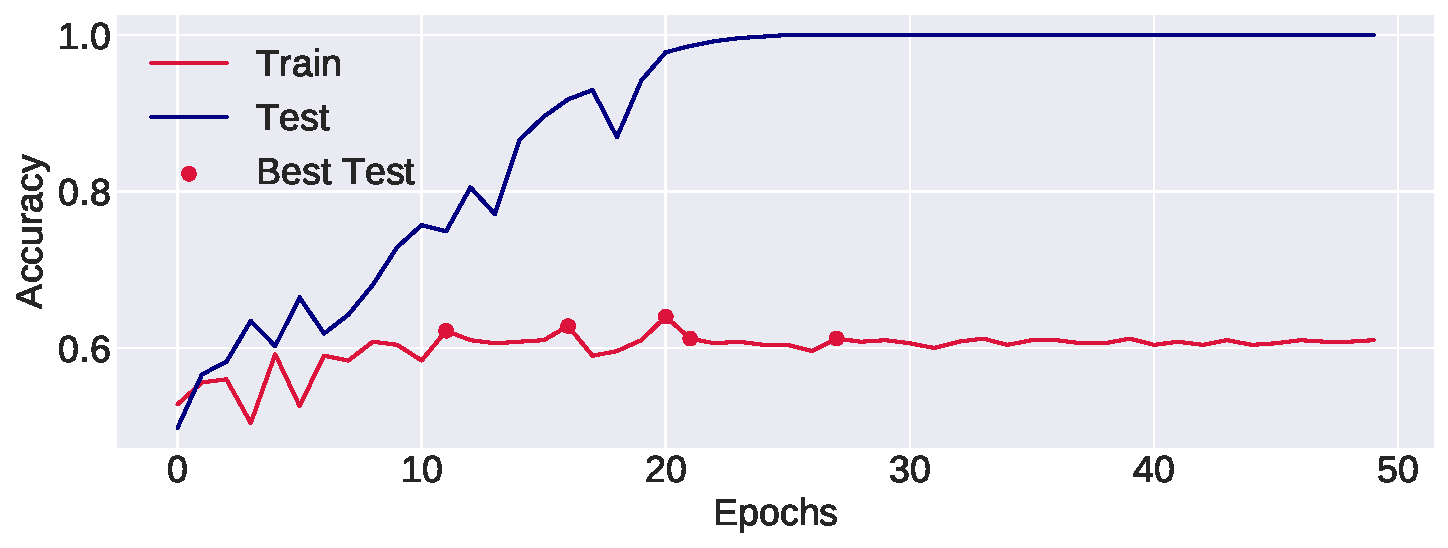
\includegraphics[scale=0.4]{../figs/hotdog_epochs.pdf}
    \caption{Figure showing the train and test accuracy of a convolutional neural network on the hot dog / not hot dog dataset.}
    \label{fig:hotdog_epochs}
\end{figure}

\section{Additional human error plot}\label{abend:human_error}

\begin{figure}[H]
    \centering
    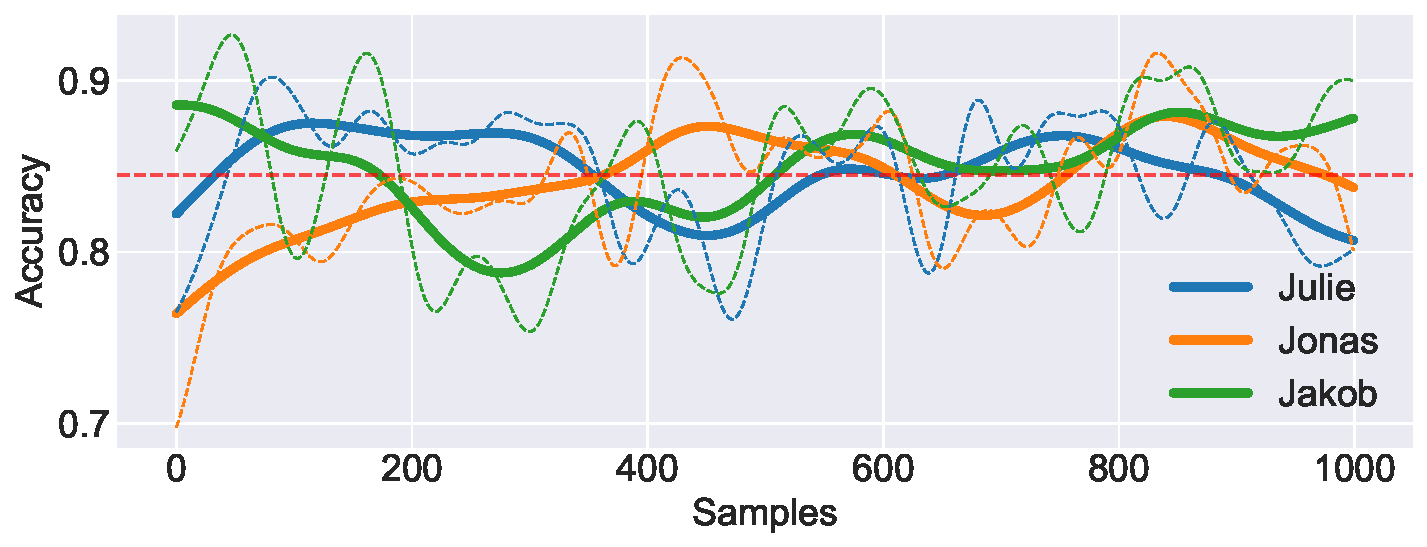
\includegraphics[scale=0.4]{figs/human_window.pdf}
    \caption{Plot showing the accuracy of the three authors categorization runs of 1000 samples from the validation set. Here the average is calculated using two centered rolling Gaussian window functions of width 50 (thick lines) and 20 (dashed lines) to better visualize how the average changes throughout the samples. The total end average of $84.5\%$ is marked with the red dashed line.}
    \label{fig:human_window}
\end{figure}

\end{appendices}
\end{document}
